\documentclass[10pt,a4paper,openbib]{article}
\usepackage[utf8]{inputenc}
\usepackage{amsmath}
\usepackage{amsfonts}
\usepackage{amssymb}
\usepackage{multicol}
\usepackage{graphicx}
\usepackage{mathtools}
\usepackage{natbib}
\usepackage{url}
\usepackage{float}
\usepackage[margin=1.5cm]{geometry}
\author{Helen Harman, \\Aberystwyth University, \\heh14@aber.ac.uk,\\ Student Number : 110007212}
\title{Can you use Viola-Jones face detection for counting people?}


\begin{document}

\maketitle

\section*{\vspace{-1.2cm} }
\textbf{Abstract:} This report discusses the face detection method described in the Viola and Jones paper ``Robust Real-Time Face Detection"\cite{violaJones}. The report will also try to address the issues involved with counting people in real-time situations. The report covers how well the Viola-Jones face detection framework works and how it can be applied to the scenario. How well combined the face detection framework with additional vision techniques to solve the issues with counting people, will be discussed. 

\begin{multicols}{2}
\section{Introduction}
The Viola-Jones paper\cite{violaJones} describes a method of detecting faces in real-time. To do this we would need to have small computation times, while still retaining high detection rates. The paper\cite{violaJones} discusses methods that try to overcome problems with false positives and false negatives detections. The Viola-Jones paper\cite{violaJones} concentrates on detecting faces, but the same principles can be used to detect other objects. \\

\noindent Face detection technologies would be useful in many situations and would help to automatise many tasks. On social networking sites tagging users in images can be done using face detection followed by face recognition. When you upload many images it is a laborious task to go through and tag all the people within the image. If can also be used for events when the number of people attending need to be counted. \\

\noindent We can also use face detection in many of our portable devices to save power. If we are not looking at our device then we can turn the screen off. \cite{exampleUse} discusses the different situations that face detection would be useful. Face recognition could be used to unlock our deceives but to do this we need to be able to first detect the presents of a face. \\

\noindent Though face detection can be used for many situations the article will concentrate on using it to count people. One of the main problems with face detection is that everyone's face is different. This means if we train an algorithm only using one person's face, it will not be able to detect everyone's face. So we have to look for what similar features faces all have. If we use images that are extremely different we run the risk of introducing a higher false positives rate, through not having enough matching features being discovered within the training set. We also do not want to cause an large amount of false negatives through having too many features. \\

\noindent The Viola-Jones paper\cite{violaJones} brings together three ideas that to try to combat these issues. These are the use of an integral image using rectangle feature detection; an adapted version of the AdaBoost machine learning algorithm; and a cascade classifier. \\

\noindent An integral image is used in calculating the rectangle features and is used to speed up the computational time. We can sum up the pixels within regions of the image, and then use this to calculate the sum of pixels within sub-regions of an image. This means that fewer operations are needed to calculate the total pixel value for sub-regions. We will have an overcomplete set of rectangle features for an image. Features rather than pixels are used to improve the computational time. \\

\noindent The second idea the Viola-Jones paper~\cite{violaJones} discusses is the use of a variation of AdaBoost to create the Haar classifier. AdaBoost is a machine learning algorithm that that looks at a set of training images and creates \cite{violaJones} ``a collection of weak classification functions to form a stronger classification". This combined with a threshold creates a strong classifier. \\

\noindent Figure~\ref{fig:violaJones} shows an example of two rectangle features that the AdaBoost algorithm has discovered faces have. The eyes have a lower intensity than the area just bellow the eyes. The nose area has a higher intensity than the eyes. These features are common across all the faces in the training data set, so will be used in the final rectangle feature detector. \\

\noindent The third idea combines these rectangle features to create a cascade of classifiers. At each level of the cascade classifier, images that do not adhere to the classifier are discarded, therefore they are not evaluated by the next classifier. Each level of the classifier has similar complexity. The classifiers have been ordered so that as many images as possible are rejected during the first levels. This helps to improve the computational time at each level.  \\

\noindent Using this version of the AdaBoost learning algorithm means that the training for the cascade classifier takes a large amount of computational time. The larger the set of training images the longer this is going to take. As the computational time as been put into creating the classifiers, less computational time is needed during the actual detection time.

\begin{figure}[H]
\begin{center}
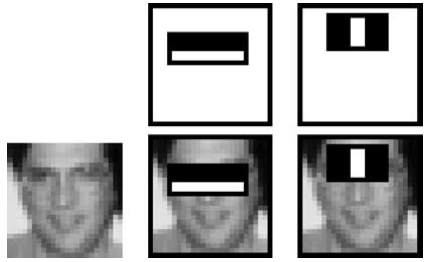
\includegraphics[scale=0.52]{images/violaJones.png} 
\caption{This image is from the Viola-Jones paper\cite{violaJones}. Shows example of rectangle-features discovered using the AdaBoost machine learning algorithm.  }
\label{fig:violaJones}
\end{center}
\end{figure}

\section{Critique of the proposed method}

After running the face detection described in the Viola-Jones paper\cite{violaJones} (using code from \cite{faceCode}), I experienced similar issues to those described in the paper\cite{violaJones}. I ran the face detection on several images of varying quality and on the input from a webcam. This section will discuss the issues the paper highlights, and my experiences of running the face detection framework using OpenCV. 

\subsection{False Positives}
The face detection framework uses rectangle feature detection on grey-scale images. The pixel intensity of rectangle areas is compared to adjacent rectangle areas to detect regions of a face. This means that areas that have similar regions of intensity as faces, also get detected. Within figure~\ref{fig:faceDetect} there is an example of a false positive being detected. The image contains a horizontal box with a light in the middle which the algorithm thinks is the eye/nose region of a face.\\

\noindent As the face detection framework just uses the intensity of pixels, anything that looks even slightly like a face gets detected as a face. This means that a drawing of a face will get detected. This is going to greatly increase the number of false positives that are found. As you can see in figure~\ref{fig:faceDrawing} the drawing of a face has been detected. 

\begin{figure}[H]
\begin{center}
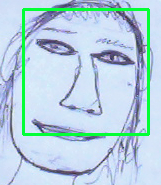
\includegraphics[scale=0.4]{images/faceDrawing.png} 
\caption{Face detection from webcam. The Viola-Jones face detection framework implemented using OpenCV~\cite{faceCode}, will find a drawing of a face.}
\label{fig:faceDrawing}
\end{center}
\end{figure}

\subsection{Angle of faces}

The face detection only works on front facing upright faces. Looking at the example training images in the paper \cite{violaJones}, only faces that follow this have been used to train the classification cascade. With a different set of training images side facing faces might be able to be detected. Faces from the side would have a significantly different set of rectangle features. This would mean a different cascade classifier would be needed otherwise less common features would be detected, so the set of classifiers would pick up a large amount of false positives. Figure~\ref{fig:faceMaxAngle} shows how the angle of a face can have an effect on whether the face is detected or not. \\

\noindent Addition step could be added to try and find faces that are not the right way up. Several rotations of the image could be pass to the framework. If faces that are 15 degrees off vertical can be detected then 12 versions of the same image at different angles would be required. This is likely to greatly increase the computational time. At the first level the classifier's computational time would increase by a factor of 12. Depending on the amount of images this level removes, the computational time of the next level should increase by a smaller factor. \\

\noindent The paper\cite{violaJones} claims that when faces are tilted $\pm$15 degrees in plane, they are not detected. From my experiments I found that the detection of faces tilted in plane is better than this and is at about $\pm$30 degrees faces stop being detected. 

\begin{figure}[H]
\begin{center}
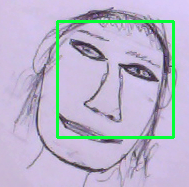
\includegraphics[scale=0.4]{images/maxAngle.png} 
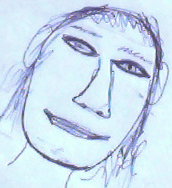
\includegraphics[scale=0.4]{images/overMaxAngle.png} 
\caption{Face detection from webcam. Shows the maximum angle at which a face can be detected. }
\label{fig:faceMaxAngle}
\end{center}
\end{figure}

\subsection{Occluded view}

If the eyes are occluded from the image then the face may not be detected but if the mouth is occluded the face should still be detected. This will increase the amount of false negatives that are detected. Figure~\ref{fig:faceHidenEye} shows that when an eye is covered-up the face is no longer detected. While using the face detection I found that even covering up a person's mouth would mean the face is not detected. It is likely that changing the threshold I used would improve the detection for when a mouth is occluded, but may also increase false positives detection rate.

\begin{figure}[H]
\begin{center}
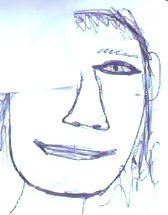
\includegraphics[scale=0.4]{images/occlusions.png} 
\caption{Will not find a face when an eye is occluded. (Uses a scale factor of 1.1)}
\label{fig:faceHidenEye}
\end{center}
\end{figure}

\subsection{Lighting}

Features are calculated using the difference in intensity of regions within an grey-scale image. This means that under certain lighting conditions faces will not be able to be detected. With a light background and a face under shadow the face is unlikely to be detected.  I found that faces with lots of shadows or lots of light shining directly onto the face could not be detected. As you can see in figure~\ref{fig:faceDetect} several faces have not been detected due to the amount of shadow covering these faces.

\subsection{Low Image Quality}
When running the OpenCV code\cite{faceCode} I found that with lower quality images I had to make the scale factor a lot smaller. This then caused a lot more false positives to be picked up. Even with a scale factor of 1.05 most the faces where not discovered. For the scenario we are are likely to be using CCTV which tends to give poor quality video. \\

\noindent As you can see in figure~\ref{fig:faceDetect} only 7 of the 12 front facing faces have been detected. For the other faces the image is off too poor a quality (or they are in lots of shadow) for the detection algorithm to detect them. CCTV camera is likely to have just as low a quality giving a similar false negative rate. 

\begin{figure}[H]
\begin{center}
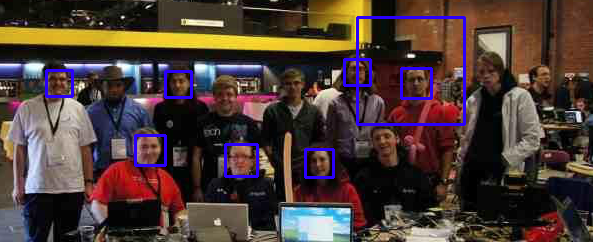
\includegraphics[scale=0.4]{images/plainFaceDetection.png} 
\caption{Face detection showing examples of false negatives and a false positive, as well as correctly detected faces.}
\label{fig:faceDetect}
\end{center}
\end{figure}

\subsection{Use of framework for other types of detection}

The Viola-Jones face detection framework can be applied to detecting other objects within images, by training a Haar classifier. A Haar classifier XML file that allows the detection of eyes is available with OpenCV. I found that this classifier found a lot of false positives, as shown in figure~\ref{fig:eyeDetection}. Most dark areas have been picked up as eyes. With a face there are a lot of rectangle-features that can be searched for but eyes will have less rectangle-features. This means that there are many other parts of an image that contain these features. 

\begin{figure}[H]
\begin{center}
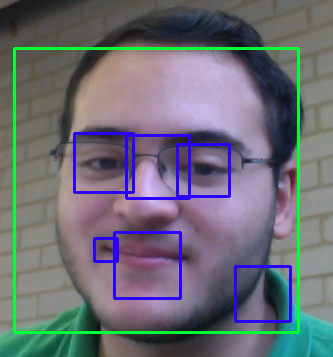
\includegraphics[scale=0.27]{images/eyeDetection.png} 
\caption{The faces that have been detected are marked by green boxes, and the eyes by blue boxes. }
\label{fig:eyeDetection}
\end{center}
\end{figure}

\subsection{Successes}
The Viola-Jones face detection has fast computational times. A long computational time has been given to the training of the Haar classifier, this has means that the detection has been simplified allowing for a shorter computational time while doing the detection. I found that on my laptop the face detection is able to work in real-time. While moving around the face detection can sometimes loose a face, but in a faction of a second it is re-detected. For counting people this would be fine as long as the same face is not counted multiple times. Face recognition could be added so that the same face is not counted multiple times. This may create addition errors, especially with low quality images.\\

\noindent As long as the faces are at the correct rotation and there is no harsh lighting then the face detection works extremely well. I am yet to find a person that it is unable to detect. This shows that the training images and algorithm have worked very well at picking up the similarities in faces. 

\section{Application of the proposed method to the scenario}
Being able to count people would be useful in many situations, from counting the number of people entering the room so that the room capacity is not reached; to counting the number of people attending an event. This section will discuss how well the proposed method works for the scenario and if additional technologies can be applied to improve the results. This includes additional software which can be used to narrow down the search area. Addition cameras and the positioning of the cameras could increase the detection rate. Other methods for detecting people will also be discussed.

\subsection{Camera Position and Number}
To use face detection for counting people, the cameras will need to be positioned at an angle that they are likely to see the front of people's faces. For example if we were to count the people entering a shop, the camera should be positioned to look at the door way. I experimented with this by setting up my webcam in a door way. I found that I had a very high false negative rate, but if the camera had been positioned differently higher detection rates would have been achieved. Having just one camera looking at the door way would mean that anyone who does not face forward would not be detected. \\

\noindent Multiple cameras could be used to capture people looking in a different direction. As someone looking 15 degrees upwards or downwards would not be detected, then two additional cameras could be used. One camera would look in a downwards angle and the other upwards. To detect faces that are out of plane, cameras positioned to the left and right would also be required. These cameras would point at angles so that people walking in diagonally can be detected. This would add extra complexity to the detection algorithm, as it would need to make sure the same person does not get counted multiple times from the different cameras. \\

\noindent For the scenario you are likely to be trying to detect people from CCTV cameras. Often the output from a CCTV cameras is very poor quality. This means that the face detection is likely to be more error prone. Using a poorer quality camera causes a lot more false negatives, so adding addition technologies may improve the detection rate.

\subsection{Using Motion}
If we want to count people going into a room then they will be moving. This means that we can narrow down the search area by first looking for motion. There are several different types of motion detection we could look at using. These include background-subtraction, dense optical flow and sparse optical flow. These methods will detect noise from other objects moving, but these other objects are not likely to look like faces or people. \\

\noindent The ``Real time Motion Detection for fast Human Identification based on face Recognition"\cite{motionDetection} paper discusses using background-subtraction and shows how a person walking through a scene can be detected. This paper does not go into how they would then use a face detection algorithm on this. The example given by the paper shows it works for a walking person without any occlusions. The paper claims the ``method has proved to be robust to detect objects in motion designed for human identification, based on face recognition"\cite{motionDetection}but does not give clear indication of what data set they have tested it on or what the actual detection rate is. \\

\noindent I found that dense optical flow does not work very well at frame rate. It also looks for movement of pixels, this would cause movement to be detected across lots of locations. A threshold can be used so that only areas with a large amount of movement are detected. The outline of people gets detected as they move across the scene, but occlusions and computational time would cause problems with this method. \\

\noindent Sparse optical flow tracks the movement of features, so works better at frame rate than dense optical flow. I found that it does not find many features on a face, but this may be due to the thresholds I was using. It did mange to pick up some features on the eyes, so the Viola-Jones\cite{violaJones} face detection could be applied to look in areas but detecting people rather than faces may improve the detection rate.\\ 

\subsection{Pedestrian detection}
People are hard to find within images, they could be anywhere within the image and in many different poses. If we are counting people walking into a shop then looking for a walking person can dramatically decrease the number of poses. We can can also decrease the area we are looking for the person in by looking for motion.\\

\noindent Dalal and Triggs's  paper\cite{dalalTriggs} on Histograms of Oriented Gradient (HOG) discusses a method for detecting people. This algorithm is an adaptation of SIFT (scale-invariant feature transform). This method works reasonably well and has good computational time. Changes to the voting method can increase the accuracy of this but unfortunately will also increase the computational time. The voting step should be run an infinite amount of to get the most accurate results possible but would take an infinite amount of time. A threshold will also have to be given to the voting, which will have an effect on the detection rate. Taking into consideration the motion within a scene could potentially decrease the computational time, and increase the detection rate\cite{dalalTriggs}. \\

\noindent A method of doing this, using a adaptation of the method discussed in Viola-Jones\cite{violaJones}, is discussed in ``Detecting Pedestrians Using Patterns of Motion and Appearance"\cite{violaJonesSnow}. This method also uses AdaBoost to train a Haar like classifier, and uses rectangle-feature detection. The classifier for this has been trained using different images from CCTV cameras and appears to achieve a reasonable good computational time. \\

\noindent Algorithms that just look for people, without looking for motion have a low detection rate due to the amount of poses that a human can be in. Just like the face detection framework rectangle features are created based on the pixel intensity within regions of the image. The difference between the two frames is used to detect the motion within the scene. This algorithm appears to work reasonably well, but still has a lot of room for improvement. \cite{violaJonesSnow}

\subsection{Different types of camera}

For this scenario as well as using person tracking instead of face tracking, using a different type of camera, or an additional camera could improve the detection results. I thought about using a thermal infra-red camera rather that a standard CCTV camera. People tend to be warmer than the surrounding areas, so you could look for a human shaped warm area. \\

\noindent A paper titled ``Improving Person Tracking Using an Inexpensive Thermal Infrared Sensor"\cite{thermal} talks about using an thermal infrared camera along with a wide-angle RGB camera. This way you can use the thermal infrared sensor to discount false positives and find false negatives. So adapting the Viola-Jones framework\cite{violaJones} for face detection to work on human detection; then looking at the output of an additional thermal infrared camera, could provided improved detection results and would still hopefully work in real-time.\\

\noindent With this method things that look like a person but aren't, for example a drawing of a person, should get discounted. Things that look human but don't have the same thermal properties of a human will not be detected. If a human is being occluded by an object the thermal sensor may still be able to pick up the thermal properties and therefore is more likely to still be able to detect the person. 

\subsection{Dealing with Occlusions}
As discussed in section 2.3, occlusions are often the cause of false negatives. The \cite{occlusions} paper discusses several methods with dealing with occlusions. One of these methods is to use a feature matrix and removes areas that the occlusions are like to be, and then checks for a partial match. \\

 \noindent A trade off between detection rate and the computation time would have too be made. With the extra processing more computation time will be taken. Also more none faces may look like part of a face, so more false positives could be detected. Combining this with pedestrian tracking may improve the detection rate but will increase the computational time.
 
 \subsection{Coloured Images and Specular Reflection}
In the Viola-Jones paper\cite{violaJones} only grey-scale images are being used but consideration should be given to the use of coloured images. For the scenario a RGB CCTV camera could be used. If we then use a training set with different skin colours under different lighting, we could try to detect areas of images that are skin coloured. \\
 
 \noindent We could also get the specular or diffuse reflection of skin.\cite{specularRefelection} All skin should have similar specular reflection properties, so if specular reflection can be detected we can detect skin. Challenges with the lighting used in the environment would have to be overcome. Christlein et al\cite{faceRec} have found when using specular reflection it is easier if you are able to control the lighting of the environment. So for indoor areas it could be considered for detecting people, but is unlikely to work well outdoors. Specular reflection can also be used in face recognition so could be used to prevent the same person being counted multiple times. This method is likely to take too much computational time for working with a real-time application.  

\section{Conclusion}
The face detection framework discussed in the paper\cite{violaJones} alone is not enough to solve the scenario of counting people. It can be improved through the use of additional cameras and the use of different types of cameras or sensors. Using methods to detect people rather than faces may improve the results. \\

\noindent Some of the further experiments that should be performed are:
\begin{itemize}
\item Positioning of the cameras
\item Number of cameras
\item The use of different types of cameras and sensors 
\item Measuring the specular reflection of areas of the face
\item The different methods that deal with occlusions (described by Azeem et al.  \cite{occlusions})
\item Detecting people or parts of people, rather than just faces.
\end{itemize}

\noindent Combining the use of the these different technique and hardware components could give high detection rates for counting people. Unfortunately combining these different methods is likely to also greatly increase the computational time. A decision on the trade off between computation time and detection rate will have to be made. \\

\noindent While writing this document I also read \cite[655-684]{book} this gave me a clearer incite into how the Viola-Jone face detection framework works. I also learnt about some of the other papers referenced in this document from this book\cite[655-684]{book}. I also read a tutorial on how to train your own Haar classifier\cite{banana}.

\section{Self-evaluation}
The first time I read the Viola-Jones paper\cite{violaJones} I did not gain a clear understanding of all the points it discusses. I then read it again a few weeks later and managed to understand the majority of the paper. I was worried about not understanding the more mathematical parts of the paper, but after breaking the math equations down they are not as hard as I first thought. I have also read and understood several other papers, which are listed in the references section. \\

\noindent Section 3 is lacking in details about how well the technologies discussed work for the given scenario, as I have not performed any experiments with them. My experiment with using a webcam pointed at a door way could have been greatly improved by trying to find a different place to put the webcam. So this article lacks any values for the detection rate or computational time for any of the algorithms discussed. This article could be improved with more conclusive results. I also should have focused more on certain points more rather than giving a brief view on lots of points. \\

\noindent I would give the following marks to each section: Introduction: 16; Critique of the proposed method: 19; Application of the proposed method to the scenario: 17; Conclusion: 7; Self-evaluation: 4; and  Bibliography: 8. With an overall mark of about 71\%(A-).  
\end{multicols}

\bibliographystyle{plain}
\bibliography{references}

\end{document}